\section{GtkListView}\label{gtklistview}

GTK 4 has added new list objects GtkListView, GtkGridView and
GtkColumnView. The new feature is described in
\href{https://docs.gtk.org/gtk4/section-list-widget.html}{Gtk API
Reference -- List Widget Overview}.

GTK 4 has other means to implement lists. They are GtkListBox and
GtkTreeView which are took over from GTK 3. There's an article in
\href{https://blog.gtk.org/2020/06/07/scalable-lists-in-gtk-4/}{Gtk
Development blog} about list widgets by Matthias Clasen. He described
why GtkListView are developed to replace GtkTreeView. GtkTreeView is
deprecated since version 4.10.

GtkListView, GtkGridView, GtkColumnView and related objects are
described in Section 29 to 33.

\subsection{Outline}\label{outline}

A list is a sequential data structure. For example, an ordered string
sequence ``one'', ``two'', ``three'', ``four'' is a list. Each element
is called item. A list is like an array, but in many cases it is
implemented with pointers which point to the next items of the list. And
it has a start point. So, each item can be referred by the index of the
item (first item, second item, \ldots, nth item, \ldots). There are two
cases. The one is the index starts from one (one-based) and the other is
from zero (zero-based).

Gio provides GListModel interface. It is a zero-based list and its items
are the same type of GObject descendants, or objects that implement the
same interface. An object implements GListModel is not a widget. So, the
list is not displayed on the screen directly. There's another object
GtkListView which is a widget to display the list. The items in the list
need to be connected to the items in GtkListView. GtkListItemFactory
instance maps items in the list to GtkListView.

\begin{figure}
\centering
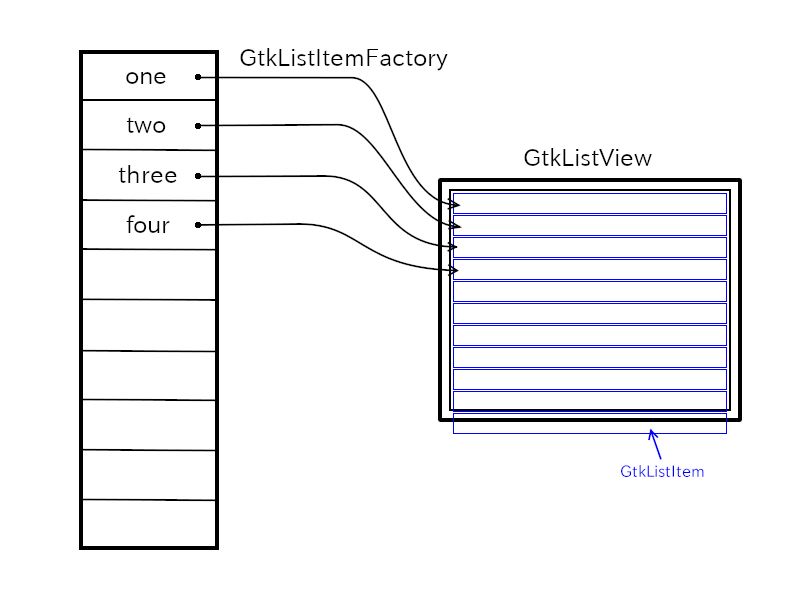
\includegraphics[width=10cm,height=7.5cm]{../image/list.png}
\caption{List}
\end{figure}

\subsection{GListModel and
GtkStringList}\label{glistmodel-and-gtkstringlist}

If you want to make a list of strings with GListModel, for example,
``one'', ``two'', ``three'', ``four'', note that strings can't be items
of the list. Because GListModel is a list of GObject objects and strings
aren't GObject objects. The word ``GObject'' here means ``GObject class
or its descendant class''. So, you need a wrapper which is a GObject and
contains a string. GtkStringObject is the wrapper object and
GtkStringList, implements GListModel, is a list of GtkStringObject.

\begin{lstlisting}[language=C]
char *array[] = {"one", "two", "three", "four", NULL};
GtkStringList *stringlist = gtk_string_list_new ((const char * const *) array);
\end{lstlisting}

The function \passthrough{\lstinline!gtk\_string\_list\_new!} creates a
GtkStringList object. Its items are GtkStringObject objects which
contain the strings ``one'', ``two'', ``three'' and ``four''. There are
functions to add items to the list or remove items from the list.

\begin{itemize}
\tightlist
\item
  \passthrough{\lstinline!gtk\_string\_list\_append!} appends an item to
  the list
\item
  \passthrough{\lstinline!gtk\_string\_list\_remove!} removes an item
  from the list
\item
  \passthrough{\lstinline!gtk\_string\_list\_get\_string!} gets a string
  in the list
\end{itemize}

See \href{https://docs.gtk.org/gtk4/class.StringList.html}{GTK 4 API
Reference -- GtkStringList} for further information.

Other list objects will be explained later.

\subsection{GtkSelectionModel}\label{gtkselectionmodel}

GtkSelectionModel is an interface to support for selections. Thanks to
this model, user can select items by clicking on them. It is implemented
by GtkMultiSelection, GtkNoSelection and GtkSingleSelection objects.
These three objects are usually enough to build an application. They are
created with another GListModel. You can also create them alone and add
a GListModel later.

\begin{itemize}
\tightlist
\item
  GtkMultiSelection supports multiple selection.
\item
  GtkNoSelection supports no selection. This is a wrapper to GListModel
  when GtkSelectionModel is needed.
\item
  GtkSingleSelection supports single selection.
\end{itemize}

\subsection{GtkListView}\label{gtklistview-1}

GtkListView is a widget to show GListModel items. GtkListItem is used by
GtkListView to represent items of a list model. But, GtkListItem itself
is not a widget, so a user needs to set a widget, for example GtkLabel,
as a child of GtkListItem to display an item of the list model. ``item''
property of GtkListItem points an object that belongs to the list model.

\begin{figure}
\centering
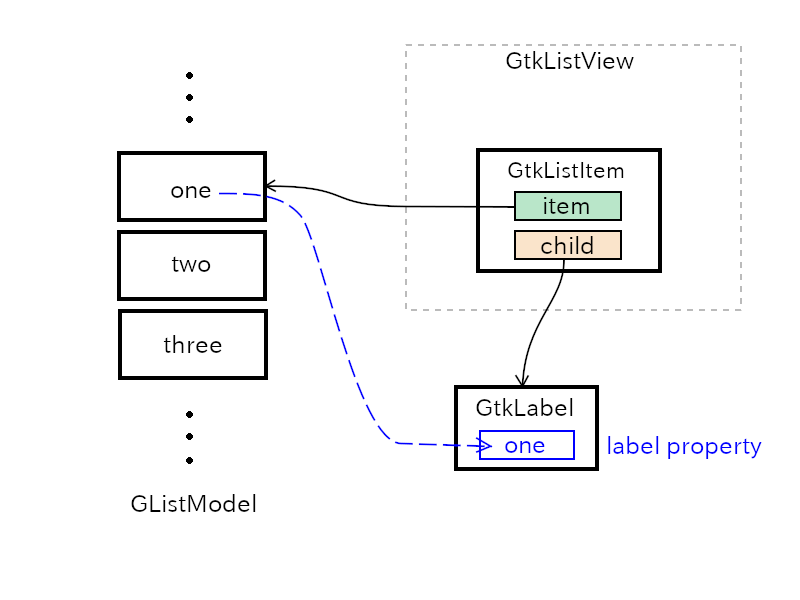
\includegraphics[width=10cm,height=7.5cm]{../image/gtklistitem.png}
\caption{GtkListItem}
\end{figure}

In case the number of items is very big, for example more than a
thousand, GtkListItem is recycled and connected to another item which is
newly displayed. This recycle makes the number of GtkListItem objects
fairly small, less than 200. This is very effective to restrain the
growth of memory consumption so that GListModel can contain lots of
items, for example, more than a million items.

\subsection{GtkListItemFactory}\label{gtklistitemfactory}

GtkListItemFactory creates or recycles GtkListItem and connects it with
an item of the list model. There are two child classes of this factory,
GtkSignalListItemFactory and GtkBuilderListItemFactory.

\subsubsection{GtkSignalListItemFactory}\label{gtksignallistitemfactory}

GtkSignalListItemFactory provides signals for users to configure a
GtkListItem object. There are four signals.

\begin{enumerate}
\def\labelenumi{\arabic{enumi}.}
\tightlist
\item
  ``setup'' is emitted to set up GtkListItem object. A user sets its
  child widget in the handler. For example, creates a GtkLabel widget
  and sets the child property of the GtkListItem to it. This setting is
  kept even the GtkListItem instance is recycled (to bind to another
  item of GListModel).
\item
  ``bind'' is emitted to bind an item in the list model to the widget.
  For example, a user gets the item from ``item'' property of the
  GtkListItem instance. Then gets the string of the item and sets the
  label property of the GtkLabel instance with the string. This signal
  is emitted when the GtkListItem is newly created, recycled or some
  changes has happened to the item of the list.
\item
  ``unbind'' is emitted to unbind an item. A user undoes everything done
  in step 2 in the signal handler. If some object are created in step 2,
  they must be destroyed.
\item
  ``teardown'' is emitted to undo everything done in step 1. So, the
  widget created in step 1 must be destroyed. After this signal, the
  list item will be destroyed.
\end{enumerate}

The following program \passthrough{\lstinline!list1.c!} shows the list
of strings ``one'', ``two'', ``three'' and ``four''. GtkNoSelection is
used, so user can't select any item.

\begin{lstlisting}[language=C, numbers=left]
#include <gtk/gtk.h>

static void
setup_cb (GtkSignalListItemFactory *self, GtkListItem *listitem, gpointer user_data) {
  GtkWidget *lb = gtk_label_new (NULL);
  gtk_list_item_set_child (listitem, lb);
  /* Because gtk_list_item_set_child sunk the floating reference of lb, releasing (unref) isn't necessary for lb. */
}

static void
bind_cb (GtkSignalListItemFactory *self, GtkListItem *listitem, gpointer user_data) {
  GtkWidget *lb = gtk_list_item_get_child (listitem);
  /* Strobj is owned by the instance. Caller mustn't change or destroy it. */
  GtkStringObject *strobj = gtk_list_item_get_item (listitem);
  /* The string returned by gtk_string_object_get_string is owned by the instance. */
  gtk_label_set_text (GTK_LABEL (lb), gtk_string_object_get_string (strobj));
}

static void
unbind_cb (GtkSignalListItemFactory *self, GtkListItem *listitem, gpointer user_data) {
  /* There's nothing to do here. */
}

static void
teardown_cb (GtkSignalListItemFactory *self, GtkListItem *listitem, gpointer user_data) {
  /* There's nothing to do here. */
  /* GtkListItem instance will be destroyed soon. You don't need to set the child to NULL. */
}

static void
app_activate (GApplication *application) {
  GtkApplication *app = GTK_APPLICATION (application);
  GtkWidget *win = gtk_application_window_new (app);
  gtk_window_set_default_size (GTK_WINDOW (win), 600, 400);
  GtkWidget *scr = gtk_scrolled_window_new ();
  gtk_window_set_child (GTK_WINDOW (win), scr);

  char *array[] = {
    "one", "two", "three", "four", NULL
  };
  /* sl is owned by ns */
  /* ns and factory are owned by lv. */
  /* Therefore, you don't need to care about their destruction. */
  GtkStringList *sl =  gtk_string_list_new ((const char * const *) array);
  GtkNoSelection *ns =  gtk_no_selection_new (G_LIST_MODEL (sl));

  GtkListItemFactory *factory = gtk_signal_list_item_factory_new ();
  g_signal_connect (factory, "setup", G_CALLBACK (setup_cb), NULL);
  g_signal_connect (factory, "bind", G_CALLBACK (bind_cb), NULL);
  /* The following two lines can be left out. The handlers do nothing. */
  g_signal_connect (factory, "unbind", G_CALLBACK (unbind_cb), NULL);
  g_signal_connect (factory, "teardown", G_CALLBACK (teardown_cb), NULL);

  GtkWidget *lv = gtk_list_view_new (GTK_SELECTION_MODEL (ns), factory);
  gtk_scrolled_window_set_child (GTK_SCROLLED_WINDOW (scr), lv);
  gtk_window_present (GTK_WINDOW (win));
}

/* ----- main ----- */
#define APPLICATION_ID "com.github.ToshioCP.list1"

int
main (int argc, char **argv) {
  GtkApplication *app;
  int stat;

  app = gtk_application_new (APPLICATION_ID, G_APPLICATION_DEFAULT_FLAGS);

  g_signal_connect (app, "activate", G_CALLBACK (app_activate), NULL);

  stat =g_application_run (G_APPLICATION (app), argc, argv);
  g_object_unref (app);
  return stat;
}
\end{lstlisting}

The file \passthrough{\lstinline!list1.c!} is located under the
directory src/misc. Make a shell script below and save it to your bin
directory, for example \passthrough{\lstinline!$HOME/bin!}.

\begin{lstlisting}[language=bash]
gcc `pkg-config --cflags gtk4` $1.c `pkg-config --libs gtk4`
\end{lstlisting}

Change the current directory to the directory includes
\passthrough{\lstinline!list1.c!} and type as follows.

\begin{lstlisting}
$ chmod 755 $HOME/bin/comp # or chmod 755 (your bin directory)/comp
$ comp list1
$ ./a.out
\end{lstlisting}

Then, the following window appears.

\begin{figure}
\centering
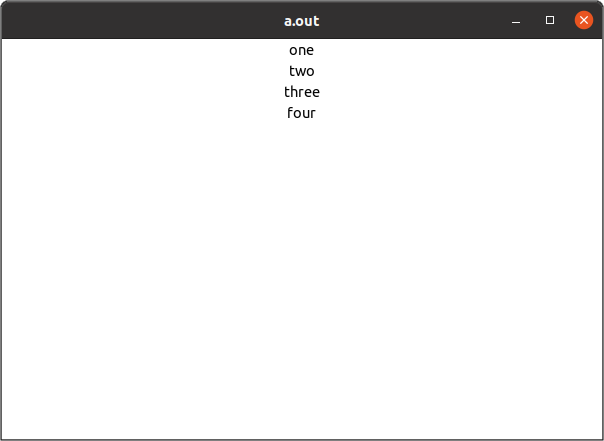
\includegraphics[width=6.04cm,height=4.4cm]{../image/list1.png}
\caption{list1}
\end{figure}

The program is not so difficult. If you feel some difficulty, read this
section again, especially GtkSignalListItemFactory subsubsection.

\subsubsection{GtkBuilderListItemFactory}\label{gtkbuilderlistitemfactory}

GtkBuilderListItemFactory is another GtkListItemFactory. Its behavior is
defined with ui file.

\begin{lstlisting}[language=XML]
<interface>
  <template class="GtkListItem">
    <property name="child">
      <object class="GtkLabel">
        <binding name="label">
          <lookup name="string" type="GtkStringObject">
            <lookup name="item">GtkListItem</lookup>
          </lookup>
        </binding>
      </object>
    </property>
  </template>
</interface>
\end{lstlisting}

Template tag is used to define GtkListItem. And its child property is
GtkLabel object. The factory sees this template and creates GtkLabel and
sets the child property of GtkListItem. This is the same as what setup
handler of GtkSignalListItemFactory did.

Then, bind the label property of the GtkLabel to the string property of
a GtkStringObject. The string object refers to the item property of the
GtkListItem. So, the lookup tag is like this:

\begin{lstlisting}
label <- string <- GtkStringObject <- item <- GtkListItem
\end{lstlisting}

The last lookup tag has a content \passthrough{\lstinline!GtkListItem!}.
Usually, C type like \passthrough{\lstinline!GtkListItem!} doesn't
appear in the content of tags. This is a special case. There is an
explanation in the
\href{https://blog.gtk.org/2020/09/05/a-primer-on-gtklistview/}{GTK
Development Blog} by Matthias Clasen.

\begin{quote}
Remember that the classname (GtkListItem) in a ui template is used as
the ``this'' pointer referring to the object that is being instantiated.
\end{quote}

Therefore, GtkListItem instance is used as the
\passthrough{\lstinline!this!} object of the lookup tag when it is
evaluated. \passthrough{\lstinline!this!} object will be explained in
section 31.

The C source code is as follows. Its name is
\passthrough{\lstinline!list2.c!} and located under src/misc directory.

\begin{lstlisting}[language=C, numbers=left]
#include <gtk/gtk.h>

static void
app_activate (GApplication *application) {
  GtkApplication *app = GTK_APPLICATION (application);
  gtk_window_present (gtk_application_get_active_window(app));
}

static void
app_startup (GApplication *application) {
  GtkApplication *app = GTK_APPLICATION (application);
  GtkWidget *win = gtk_application_window_new (app);
  gtk_window_set_default_size (GTK_WINDOW (win), 600, 400);
  GtkWidget *scr = gtk_scrolled_window_new ();
  gtk_window_set_child (GTK_WINDOW (win), scr);

  char *array[] = {
    "one", "two", "three", "four", NULL
  };
  GtkStringList *sl = gtk_string_list_new ((const char * const *) array);
  GtkSingleSelection *ss = gtk_single_selection_new (G_LIST_MODEL (sl));

  const char *ui_string =
"<interface>"
  "<template class=\"GtkListItem\">"
    "<property name=\"child\">"
      "<object class=\"GtkLabel\">"
        "<binding name=\"label\">"
          "<lookup name=\"string\" type=\"GtkStringObject\">"
            "<lookup name=\"item\">GtkListItem</lookup>"
          "</lookup>"
        "</binding>"
      "</object>"
    "</property>"
  "</template>"
"</interface>"
;
  GBytes *gbytes = g_bytes_new_static (ui_string, strlen (ui_string));
  GtkListItemFactory *factory = gtk_builder_list_item_factory_new_from_bytes (NULL, gbytes);

  GtkWidget *lv = gtk_list_view_new (GTK_SELECTION_MODEL (ss), factory);
  gtk_scrolled_window_set_child (GTK_SCROLLED_WINDOW (scr), lv);
}

/* ----- main ----- */
#define APPLICATION_ID "com.github.ToshioCP.list2"

int
main (int argc, char **argv) {
  GtkApplication *app;
  int stat;

  app = gtk_application_new (APPLICATION_ID, G_APPLICATION_DEFAULT_FLAGS);

  g_signal_connect (app, "startup", G_CALLBACK (app_startup), NULL);
  g_signal_connect (app, "activate", G_CALLBACK (app_activate), NULL);

  stat =g_application_run (G_APPLICATION (app), argc, argv);
  g_object_unref (app);
  return stat;
}
\end{lstlisting}

No signal handler is needed for GtkBulderListItemFactory.
GtkSingleSelection is used, so user can select one item at a time.

Because this is a small program, the ui data is given as a string.

\subsection{GtkDirectoryList}\label{gtkdirectorylist}

GtkDirectoryList is a list model containing GFileInfo objects which are
information of files under a certain directory. It uses
\passthrough{\lstinline!g\_file\_enumerate\_children\_async()!} to get
the GFileInfo objects. The list model is created by
\passthrough{\lstinline!gtk\_directory\_list\_new!} function.

\begin{lstlisting}[language=C]
GtkDirectoryList *gtk_directory_list_new (const char *attributes, GFile *file);
\end{lstlisting}

\passthrough{\lstinline!attributes!} is a comma separated list of file
attributes. File attributes are key-value pairs. A key consists of a
namespace and a name. For example, ``standard::name'' key is the name of
a file. ``standard'' means general file information. ``name'' means
filename. The following table shows some example.

\begin{longtable}[]{@{}
  >{\raggedright\arraybackslash}p{(\columnwidth - 2\tabcolsep) * \real{0.1905}}
  >{\raggedright\arraybackslash}p{(\columnwidth - 2\tabcolsep) * \real{0.8095}}@{}}
\toprule\noalign{}
\begin{minipage}[b]{\linewidth}\raggedright
key
\end{minipage} & \begin{minipage}[b]{\linewidth}\raggedright
meaning
\end{minipage} \\
\midrule\noalign{}
\endhead
\bottomrule\noalign{}
\endlastfoot
standard::type & file type. for example, regular file, directory,
symbolic link, etc. \\
standard::name & filename \\
standard::size & file size in bytes \\
access::can-read & read privilege if the user is able to read the
file \\
time::modified & the time the file was last modified in seconds since
the UNIX epoch \\
\end{longtable}

The current directory is ``.''. The following program makes
GtkDirectoryList \passthrough{\lstinline!dl!} and its contents are
GFileInfo objects under the current directory.

\begin{lstlisting}[language=C]
GFile *file = g_file_new_for_path (".");
GtkDirectoryList *dl = gtk_directory_list_new ("standard::name", file);
g_object_unref (file);
\end{lstlisting}

It is not so difficult to make file listing program by changing
\passthrough{\lstinline!list2.c!} in the previous subsection. One
problem is that GInfoFile doesn't have properties. Lookup tag look for a
property, so it is useless for looking for a filename from a GFileInfo
object. Instead, closure tag is appropriate in this case. Closure tag
specifies a function and the type of the return value of the function.

\begin{lstlisting}[language=C]
char *
get_file_name (GtkListItem *item, GFileInfo *info) {
  return G_IS_FILE_INFO (info) ? g_strdup (g_file_info_get_name (info)) : NULL;
}
... ...
... ...

"<interface>"
  "<template class=\"GtkListItem\">"
    "<property name=\"child\">"
      "<object class=\"GtkLabel\">"
        "<binding name=\"label\">"
          "<closure type=\"gchararray\" function=\"get_file_name\">"
            "<lookup name=\"item\">GtkListItem</lookup>"
          "</closure>"
        "</binding>"
      "</object>"
    "</property>"
  "</template>"
"</interface>"
\end{lstlisting}

\begin{itemize}
\tightlist
\item
  The string ``gchararray'' is a type name. The type ``gchar'' is a type
  name and it is the same as C type ``char''. Therefore, ``gchararray''
  is ``an array of char type'', which is the same as string type. It is
  used to get the type of GValue object. GValue is a generic value and
  it can contain various type of values. For example, the type name can
  be gboolean, gchar (char), gint (int), gfloat (float), gdouble
  (double), gchararray (char *) and so on. These type names are the
  names of the fundamental types that are registered to the type system.
  See
  \href{https://github.com/ToshioCP/Gobject-tutorial/blob/main/gfm/sec5.md\#gvalue}{GObject
  tutorial}.
\item
  Closure tag has type attribute and function attribute. Function
  attribute specifies the function name and type attribute specifies the
  type of the return value of the function. The contents of closure tag
  (it is between \textless closure\ldots\textgreater{}
  and\textless/closure\textgreater) is parameters of the function.
  \passthrough{\lstinline!<lookup name="item">GtkListItem</lookup>!}
  gives the value of the item property of the GtkListItem. This will be
  the second argument of the function. The first parameter is always the
  GListItem instance, which is a `this' object. The `this' object is
  explained in section 31.
\item
  \passthrough{\lstinline!gtk\_file\_name!} function is the callback
  function for the closure tag. It first checks the
  \passthrough{\lstinline!info!} parameter. Because it can be NULL when
  GListItem \passthrough{\lstinline!item!} is unbounded. If it's
  GFileInfo, it returns the copied filename. Because the return value
  (filename) of \passthrough{\lstinline!g\_file\_info\_get\_name!} is
  owned by GFileInfo object. So, the the string needs to be duplicated
  to give the ownership to the caller. Binding tag binds the ``label''
  property of the GtkLabel to the closure tag.
\end{itemize}

The whole program (\passthrough{\lstinline!list3.c!}) is as follows. The
program is located in src/misc directory.

\begin{lstlisting}[language=C, numbers=left]
#include <gtk/gtk.h>

char *
get_file_name (GtkListItem *item, GFileInfo *info) {
  return G_IS_FILE_INFO (info) ? g_strdup (g_file_info_get_name (info)) : NULL;
}

static void
app_activate (GApplication *application) {
  GtkApplication *app = GTK_APPLICATION (application);
  gtk_window_present (gtk_application_get_active_window(app));
}

static void
app_startup (GApplication *application) {
  GtkApplication *app = GTK_APPLICATION (application);
  GtkWidget *win = gtk_application_window_new (app);
  gtk_window_set_default_size (GTK_WINDOW (win), 600, 400);
  GtkWidget *scr = gtk_scrolled_window_new ();
  gtk_window_set_child (GTK_WINDOW (win), scr);

  GFile *file = g_file_new_for_path (".");
  GtkDirectoryList *dl = gtk_directory_list_new ("standard::name", file);
  g_object_unref (file);
  GtkNoSelection *ns = gtk_no_selection_new (G_LIST_MODEL (dl));

  const char *ui_string =
"<interface>"
  "<template class=\"GtkListItem\">"
    "<property name=\"child\">"
      "<object class=\"GtkLabel\">"
        "<binding name=\"label\">"
          "<closure type=\"gchararray\" function=\"get_file_name\">"
            "<lookup name=\"item\">GtkListItem</lookup>"
          "</closure>"
        "</binding>"
      "</object>"
    "</property>"
  "</template>"
"</interface>"
;
  GBytes *gbytes = g_bytes_new_static (ui_string, strlen (ui_string));
  GtkListItemFactory *factory = gtk_builder_list_item_factory_new_from_bytes (NULL, gbytes);

  GtkWidget *lv = gtk_list_view_new (GTK_SELECTION_MODEL (ns), factory);
  gtk_scrolled_window_set_child (GTK_SCROLLED_WINDOW (scr), lv);
}

/* ----- main ----- */
#define APPLICATION_ID "com.github.ToshioCP.list3"

int
main (int argc, char **argv) {
  GtkApplication *app;
  int stat;

  app = gtk_application_new (APPLICATION_ID, G_APPLICATION_DEFAULT_FLAGS);

  g_signal_connect (app, "startup", G_CALLBACK (app_startup), NULL);
  g_signal_connect (app, "activate", G_CALLBACK (app_activate), NULL);

  stat =g_application_run (G_APPLICATION (app), argc, argv);
  g_object_unref (app);
  return stat;
}
\end{lstlisting}

The ui data (xml data above) is used to build the GListItem template at
runtime. GtkBuilder refers to the symbol table to find the function
\passthrough{\lstinline!get\_file\_name!}.

Generally, a symbol table is used by a linker to link objects to an
executable file. It includes function names and their location. A linker
usually doesn't put a symbol table into the created executable file. But
if \passthrough{\lstinline!--export-dynamic!} option is given, the
linker adds the symbol table to the executable file.

To accomplish it, an option
\passthrough{\lstinline!-Wl,--export-dynamic!} is given to the C
compiler.

\begin{itemize}
\tightlist
\item
  \passthrough{\lstinline!-Wl!} is a C compiler option that passes the
  following option to the linker.
\item
  \passthrough{\lstinline!--export-dynamic!} is a linker option. The
  following is cited from the linker document. ``When creating a
  dynamically linked executable, add all symbols to the dynamic symbol
  table. The dynamic symbol table is the set of symbols which are
  visible from dynamic objects at run time.''
\end{itemize}

Compile and execute it.

\begin{lstlisting}
$ gcc -Wl,--export-dynamic `pkg-config --cflags gtk4` list3.c `pkg-config --libs gtk4`
\end{lstlisting}

You can also make a shell script to compile
\passthrough{\lstinline!list3.c!}

\begin{lstlisting}[language=bash]
gcc -Wl,--export-dynamic `pkg-config --cflags gtk4` $1.c `pkg-config --libs gtk4`
\end{lstlisting}

Save this one liner to a file \passthrough{\lstinline!comp!}. Then, copy
it to \passthrough{\lstinline!$HOME/bin!} and give it executable
permission.

\begin{lstlisting}
$ cp comp $HOME/bin/comp
$ chmod +x $HOME/bin/comp
\end{lstlisting}

You can compile \passthrough{\lstinline!list3.c!} and execute it, like
this:

\begin{lstlisting}
$ comp list3
$ ./a.out
\end{lstlisting}

\begin{figure}
\centering
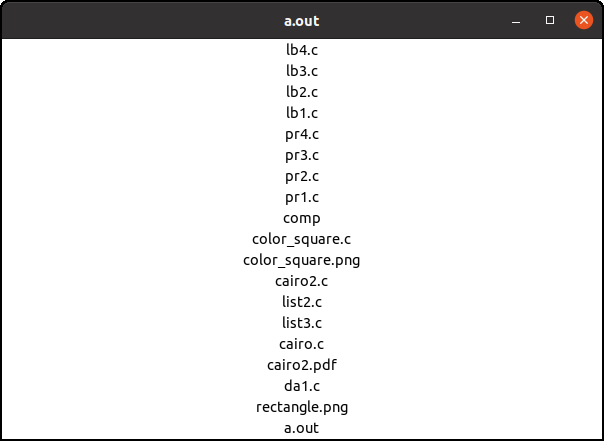
\includegraphics[width=10cm,height=7.3cm]{../image/list3.png}
\caption{screenshot list3}
\end{figure}
